\makeatletter
\def\input@path{{./tuc2019/beamer/}}
\makeatother
\documentclass[10pt]{beamer}
\usetheme[fakcolor=if]{tuc2019}

\usepackage{pgffor}
\usepackage{tikz}
\usetikzlibrary{calc}
\usepackage{graphicx}


\newcommand{\CoverFromTop}[2][img]{%
	\fill[white]
	($(#1.north west)!#2!(#1.south west)$)
	rectangle
	(#1.south east);%
}

\title{Verifikation verteilter Systeme in Isabelle}
\subtitle{Ein Vergleich von Kleppmann und I/O-Automaten}
\author{Sepp Stage}
\date[\today]{}
\institute[TUC, Fak. BS]{TU Chemnitz, Fakultät Betriebssysteme}
\titlegraphic{
\includegraphics[height=0.2\textheight]{tuc2019/logo/tuc_green}}

\begin{document}
	\begingroup
	\tucthreeheadlines
	\frame{\titlepage}
	\endgroup
	
	\frame{\tableofcontents}
	
	\newpage
	\section{Einleitung}
	AT\&T
	\newpage
	\section{Das Zwei-Phase-Commit-Protokoll}
	\subsection{Übergänge des Koordinators}
	\begin{frame}
	\centering
	\foreach \i in {1,...,5}{
		\only<\i>{%
			\includegraphics[width=\textwidth,height=\textheight,keepaspectratio]{Bilder/AutomatCoord\i}
		}
	}
	\end{frame}
	
	\subsection{Übergänge eines Teilnehmers}	
	\begin{frame}
		\centering
		\foreach \i in {1,...,4}{
			\only<\i>{%
				\includegraphics[width=\textwidth,height=\textheight,keepaspectratio]{Bilder/AutomatPart\i}
			}
		}
	\end{frame}

	\newpage
	\subsection{Beispielhafte Abläufe}

	\begin{frame}[t]
		\vspace*{0pt}
		\centering
		\begin{tikzpicture}
			\node[anchor=north west,inner sep=0] (img) at (0,0) {%
				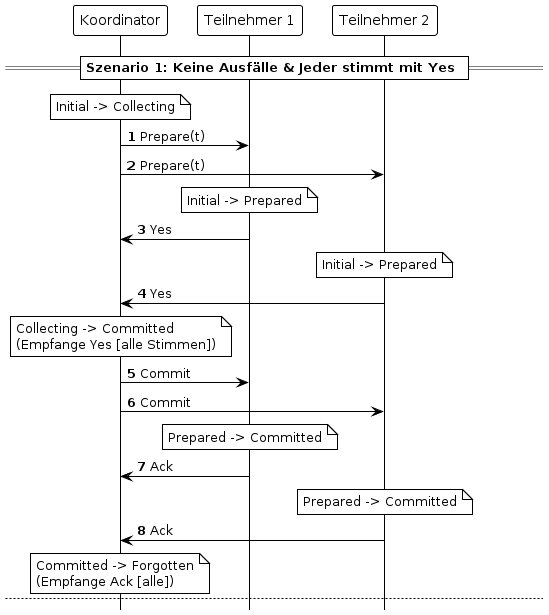
\includegraphics[width=\textwidth, height=0.98\textheight, keepaspectratio]{Bilder/Sequences/1/4}%
			};
			
			\only<1>{\CoverFromTop{0.3}}
			\only<2>{\CoverFromTop{0.51}}
			\only<3>{\CoverFromTop{0.688}}
			\only<4>{\CoverFromTop{1}}
		\end{tikzpicture}
	\end{frame}
	
	\begin{frame}[t]
		\vspace*{0pt}
		\centering
		\begin{tikzpicture}
			\node[anchor=north west,inner sep=0] (img) at (0,0) {%
				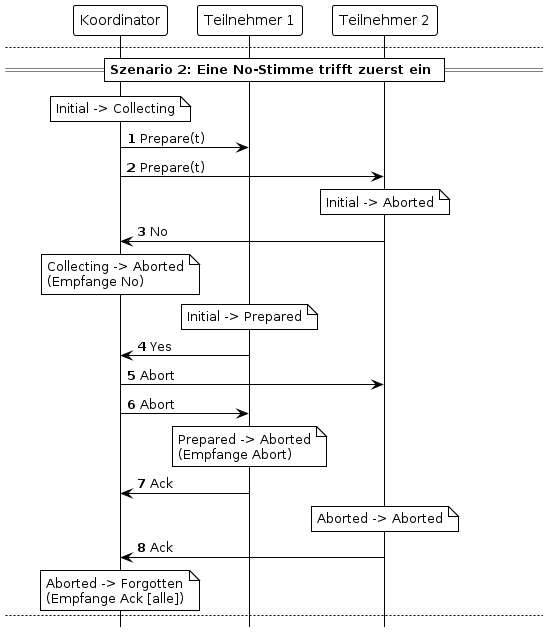
\includegraphics[width=\textwidth, height=0.98\textheight, keepaspectratio]{Bilder/Sequences/2/5}%
			};
			
			\only<1>{\CoverFromTop{0.298}}
			\only<2>{\CoverFromTop{0.4}}
			\only<3>{\CoverFromTop{0.58}}
			\only<4>{\CoverFromTop{0.67}}
			\only<5>{\CoverFromTop{1}}
		\end{tikzpicture}
	\end{frame}

	\begin{frame}[t]
		\vspace*{0pt}
		\centering
		\begin{tikzpicture}
			\node[anchor=north west,inner sep=0] (leftimg) at (0,0) {%
				
\includegraphics[width=0.49\textwidth]{Bilder/Sequences/3/2}%
			};
			\node[anchor=north west,inner sep=0] (rightimg) at (6.2cm,0) {%
				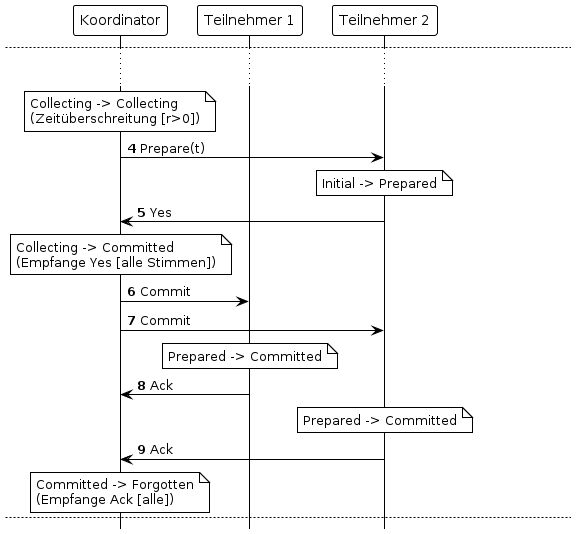
\includegraphics[width=0.49\textwidth]{Bilder/Sequences/3/6}%
			};
			
			\only<1>{\CoverFromTop[leftimg]{0.75}}
			\only<1,2>{\CoverFromTop[rightimg]{0}}
			\only<3>{\CoverFromTop[rightimg]{0.317}}
			\only<4>{\CoverFromTop[rightimg]{0.43}}
			\only<5>{\CoverFromTop[rightimg]{0.64}}
			\only<6>{\CoverFromTop[rightimg]{1}}
		\end{tikzpicture}
	\end{frame}
	
	\begin{frame}[t]
		\vspace*{0pt}
		\centering
		\begin{tikzpicture}
			\node[anchor=north west,inner sep=0] (leftimg) at (0,0) {%
				
\includegraphics[width=0.49\textwidth]{Bilder/Sequences/4/3}%
			};
			\node[anchor=north west,inner sep=0] (rightimg) at (6.2cm,0) {%
				
\includegraphics[width=0.49\textwidth]{Bilder/Sequences/4/6}%
			};
			
			\only<1>{\CoverFromTop[leftimg]{0.55}}
			\only<2>{\CoverFromTop[leftimg]{0.75}}
			\only<1-3>{\CoverFromTop[rightimg]{0}}
			\only<4>{\CoverFromTop[rightimg]{0.382}}
			\only<5>{\CoverFromTop[rightimg]{0.52}}
			\only<6>{\CoverFromTop[rightimg]{0.66}}
			\only<7>{\CoverFromTop[rightimg]{1}}
		\end{tikzpicture}
	\end{frame}
	
	\newpage
	\section{Kleppmann}
	\newpage
	\subsection{Modellvorstellung}
	\newpage
	\subsection{Invarianten}
	\newpage
	\subsection{Beweis einer Invarianten}
	\newpage
	\subsection{Beweis der einheitlichen Zustimmung}
	
	\newpage
	\section{I/O Automaten}
	\newpage
	\subsection{Modellvorstellung}
	\newpage
	\subsection{Invarianten}
	\newpage
	\subsection{Beweis einer Invarianten}
	\newpage
	\subsection{Beweis der einheitlichen Zustimmung}
	
	\newpage
	\section{Vergleich}
	\newpage
	\subsection{Kriterien...}
	
	\newpage
	\section{Fazit}
	blblblb
\end{document}